%!TEX TS-program = pdflatex                                          %
%!TEX encoding = UTF8                                                %
%!TEX spellcheck = en-US                                             %
%
%%%%%%%%%%%%%%%%%%%%%%%%%%%%%%%%%%%%%%%%%%%%%%%%%%%%%%%%%%%%%%%%%%%%%%
% Handout_ModelingStructuralLesions.tex
% A handout to follow during the hands-on sessions 
% 
% Authors: Paula Sanz Leon
% 
% 
%%%%%%%%%%%%%%%%%%%%%%%%%%%%%%%%%%%%%%%%%%%%%%%%%%%%%%%%%%%%%%%%%%%%%%
% based on the tufte-latex template                                  %

\documentclass{tufte-handout}

%\geometry{showframe}% for debugging purposes -- displays the margins

\usepackage{amsmath}

% Set up the images/graphics \underline{\textbf{Analysis}}
\usepackage{graphicx}
\setkeys{Gin}{width=\linewidth,totalheight=\textheight,keepaspectratio}
\graphicspath{{figures/}}

\title{The Virtual Brain: Hands on Session \#1}
\date{7th June 2014} 

% The following package makes prettier tables.  
\usepackage{booktabs}

% 
%\usepackage{caption}
%\usepackage{subcaption}

% The units package provides nice, non-stacked fractions and better spacing
% for units.
\usepackage{units}
\usepackage[svgnames]{xcolor}

% The fancyvrb package lets us customize the formatting of verbatim
% environments.  We use a slightly smaller font.
\usepackage{fancyvrb}
\fvset{fontsize=\normalsize}

% Small sections of multiple columns
\usepackage{multicol}

% For adjustwidth environment
\usepackage[strict]{changepage}

% For formal definitions
\usepackage{framed}

% Resume a list
\usepackage{enumitem}

% Provides paragraphs of dummy text
\usepackage{lipsum}

% These commands are used to pretty-print LaTeX commands
\newcommand{\doccmd}[1]{\texttt{\textbackslash#1}}% command name -- adds backslash automatically
\newcommand{\docopt}[1]{\ensuremath{\langle}\textrm{\textit{#1}}\ensuremath{\rangle}}% optional command argument
\newcommand{\docarg}[1]{\textrm{\textit{#1}}}% (required) command argument
\newenvironment{docspec}{\begin{quote}\noindent}{\end{quote}}% command specification environment
\newcommand{\docenv}[1]{\textsf{#1}}% environment name
\newcommand{\docpkg}[1]{\texttt{#1}}% package name
\newcommand{\doccls}[1]{\texttt{#1}}% document class name
\newcommand{\docclsopt}[1]{\texttt{#1}}% document class option name

% environment derived from framed.sty: see leftbar environment definition
\definecolor{formalshade}{rgb}{0.95,0.95,1}
\definecolor{simulationshade}{rgb}{0.92, 1.0, 0.95}

\newenvironment{formal}{%
  \def\FrameCommand{%
    \hspace{1pt}%
    {\color{DarkBlue}\vrule width 2pt}%
    {\color{formalshade}\vrule width 4pt}%
    \colorbox{formalshade}%
  }%
  \MakeFramed{\advance\hsize-\width\FrameRestore}%
  \noindent\hspace{-4.55pt}% disable indenting first paragraph
  \begin{adjustwidth}{}{7pt}%
  \vspace{2pt}\vspace{2pt}%
}
{%
  \vspace{2pt}\end{adjustwidth}\endMakeFramed%
}

\newenvironment{simulation}{%
  \def\FrameCommand{%
    \hspace{1pt}%
    {\color{ForestGreen}\vrule width 2pt}%
    {\color{simulationshade}\vrule width 4pt}%
    \colorbox{simulationshade}%
  }%
  \MakeFramed{\advance\hsize-\width\FrameRestore}%
  \noindent\hspace{-4.55pt}% disable indenting first paragraph
  \begin{adjustwidth}{}{7pt}%
  \vspace{2pt}\vspace{2pt}%
}
{%
  \vspace{2pt}\end{adjustwidth}\endMakeFramed%
}

\newenvironment{blah}{%
  \def\FrameCommand{%
    \hspace{1pt}%
    {\color{DarkOrange}\vrule width 2pt}%
    {\color{PeachPuff}\vrule width 4pt}%
    \colorbox{PeachPuff}%
  }%
  \MakeFramed{\advance\hsize-\width\FrameRestore}%
  \noindent\hspace{-4.55pt}% disable indenting first paragraph
  \begin{adjustwidth}{}{7pt}%
  \vspace{2pt}\vspace{2pt}%
}
{%
  \vspace{2pt}\end{adjustwidth}\endMakeFramed%
}

\begin{document}
\maketitle % this prints the handout title, author, and date

\begin{abstract}

\noindent TVB allows for a systematic exploration and manipulation of every
underlying component of a large-scale brain network model, such as the neural
mass model governing the local dynamics or the structural connectivity
constraining the space-time structure of the network couplings.
\begin{marginfigure}%
  
\includegraphics[width=\linewidth]{tvb_logo_transparent_square}
  %\caption{TVB evil logo}
  \label{fig:marginfig}
\end{marginfigure}
\end{abstract}

%\printclassoptions

%\begin{fullwidth} % uncomment this environment to get full texwidth paragraphs 
%\textsc{The Virtual Brain} is a facilitating technology. It enables
%researchers from the domains of  computational neuroscience and medicine to
%study and focus on a particular problem, and directly build a model of the
%brain that can be tested under different scenarios. So, every time we require
%to perform a simulation for our work, we do not require to develop the
%underlying computational model.   
%\end{fullwidth}

\section{Objectives}\label{sec:objectives}

This tutorial presents the basic anatomy of a brain network model at the region level using The
Virtual Brain's (TVB's) graphical interface. Following these steps you should
be able to reproduce the results from the simulations in the project Building
Your Own Brain Network Model.

\subsection{What's inside Project Session\_I\_BuildingYourOwnBrainNetworkModel}\label{sec:project_data}

\begin{margintable}
  \centering
  \fontfamily{ppl}\selectfont
  \begin{tabular}{ll}
    \toprule
    Datatype & Sumary info                       \\
    \midrule
    Default Connectivity & 74 {nodes}            \\
    Region Time Series   & -                     \\
    Surface Time Series  & -                     \\ 
    EEG Time-Series      &                       \\
    Local Connectivity   & -                     \\
    Fourier Spectra      & -                     \\ 
    Wavelet Spectrograms & -                     \\
    \bottomrule
  \end{tabular}
  \caption{Some of the dataypes}
  \label{tab:normaltab}
\end{margintable}


% let's start a new thought -- a new section
\newthought{In this session}, due to time constraints the simulations were
already run. We'll only go through the necessary steps required to reproduce
some of the data described in Table~\ref{tab:normaltab}. You can always start
over, click along and/or try to change parameters.


\subsection{Steps: Building A Discrete Brain Network Model (region-based simulations)}\label{sec:steps}

In the \textsc{simulator} page (Fig.~\ref{fig:fig}), you could name your
simulation and directly launch it with the default parameters. However, in
this example we slightly changed the default parameters and configure some
visualizers on the right column to have a quick idea of some properties of the
simulated data.

A basic simulation at using a coarse representation of the brain consists of
five main components, each of these components is a configurable object in
TVB:

\begin{blah}
\begin{itemize}
\item Model, which is, at its core, a set of differential equations describing the local neuronal dynamics;
\item Connectivity, represents the large scale structural connectivity of the brain, ie white-matter tracts;
\item Coupling, is a function that is used to join the local Model dynamics at distinct locations over the connections described in Connectivity;
\item Integrator, is the integration scheme that will be applied to the coupled set of differential equations;
\item Monitors, one or more Monitors can be attached to a simulation, they act to record the output from the Simulator.
\end{itemize}
\end{blah}

\begin{figure}[h]
  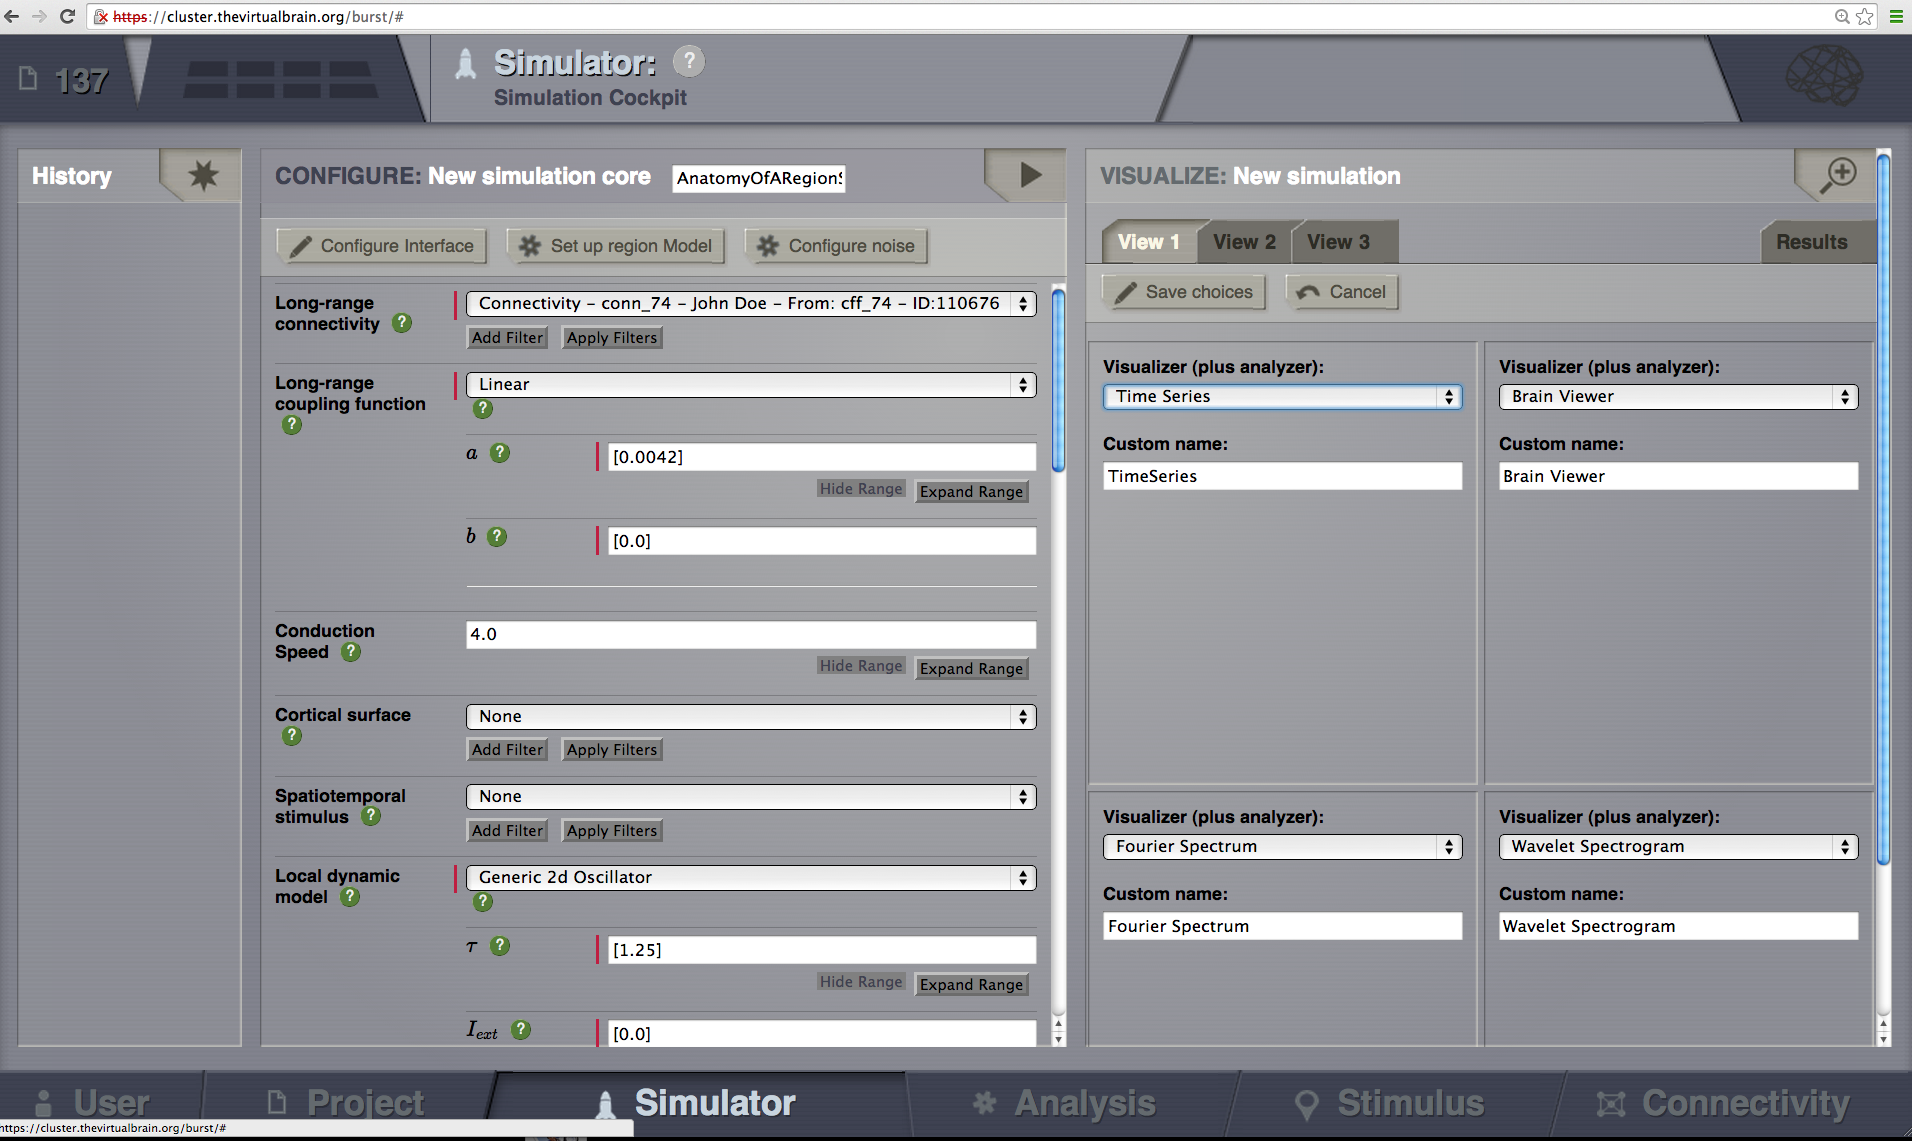
\includegraphics[width=\linewidth]{Handout_UI_BuildingYourOwnBrainNetworkModel_SimulatorArea}%
  \caption{TVB Simulator page}%
  \label{fig:fig}%
\end{figure}


\begin{simulation}
\begin{enumerate}
\item Let's start defining some structure for our network. We'll rely on TVB's default \underline{Connectivity} matrix. Having loaded the default dataset we can then alter the speed of signal propagation through the network to 4.0 $m\,s^{-1}$. 

\item Then we define a \underline{Model} for the local dynamics we wish to use, there are a number of predefined \underline{Models} available in TVB, as an example here we'll use a generic 2 dimensional oscillator. (Fig. \ref{fig:step_01}  and Table \ref{tab:modeltab}).

\item The next step is to define a \underline{Coupling} function, proper setting of the parameters for this function requires some knowledge of the properties of both the \underline{Model} being used and the structure through which it is connected. For our present purposes, we happen to know that for the parameters we just set connected through TVB's default \underline{Connectivity} matrix, a linear function with a slope of 0.0042 is a reasonable thing to use. 

\item Now that we've defined our structure and dynamics we need to select an integration scheme. 
To keep things simple, we'll use \underline{HeunDeterministic} with the default integration time step size. The most important thing here is to use a step size that is small enough for the integration to be numerically stable. Here, we chose a value of \underline{dt} equal to 0.1 ms.

\item  The last component we need to define are some \underline{Monitors}. The \underline{TemporalAverage Monitor} averages over a time window of length period returning one time point every period ms. It also, by default, only returns those state-variables flagged in the \underline{Models} definition as \underline{Variables watched by Monitors}
\end{enumerate}
\end{simulation}

\begin{figure}[h]
  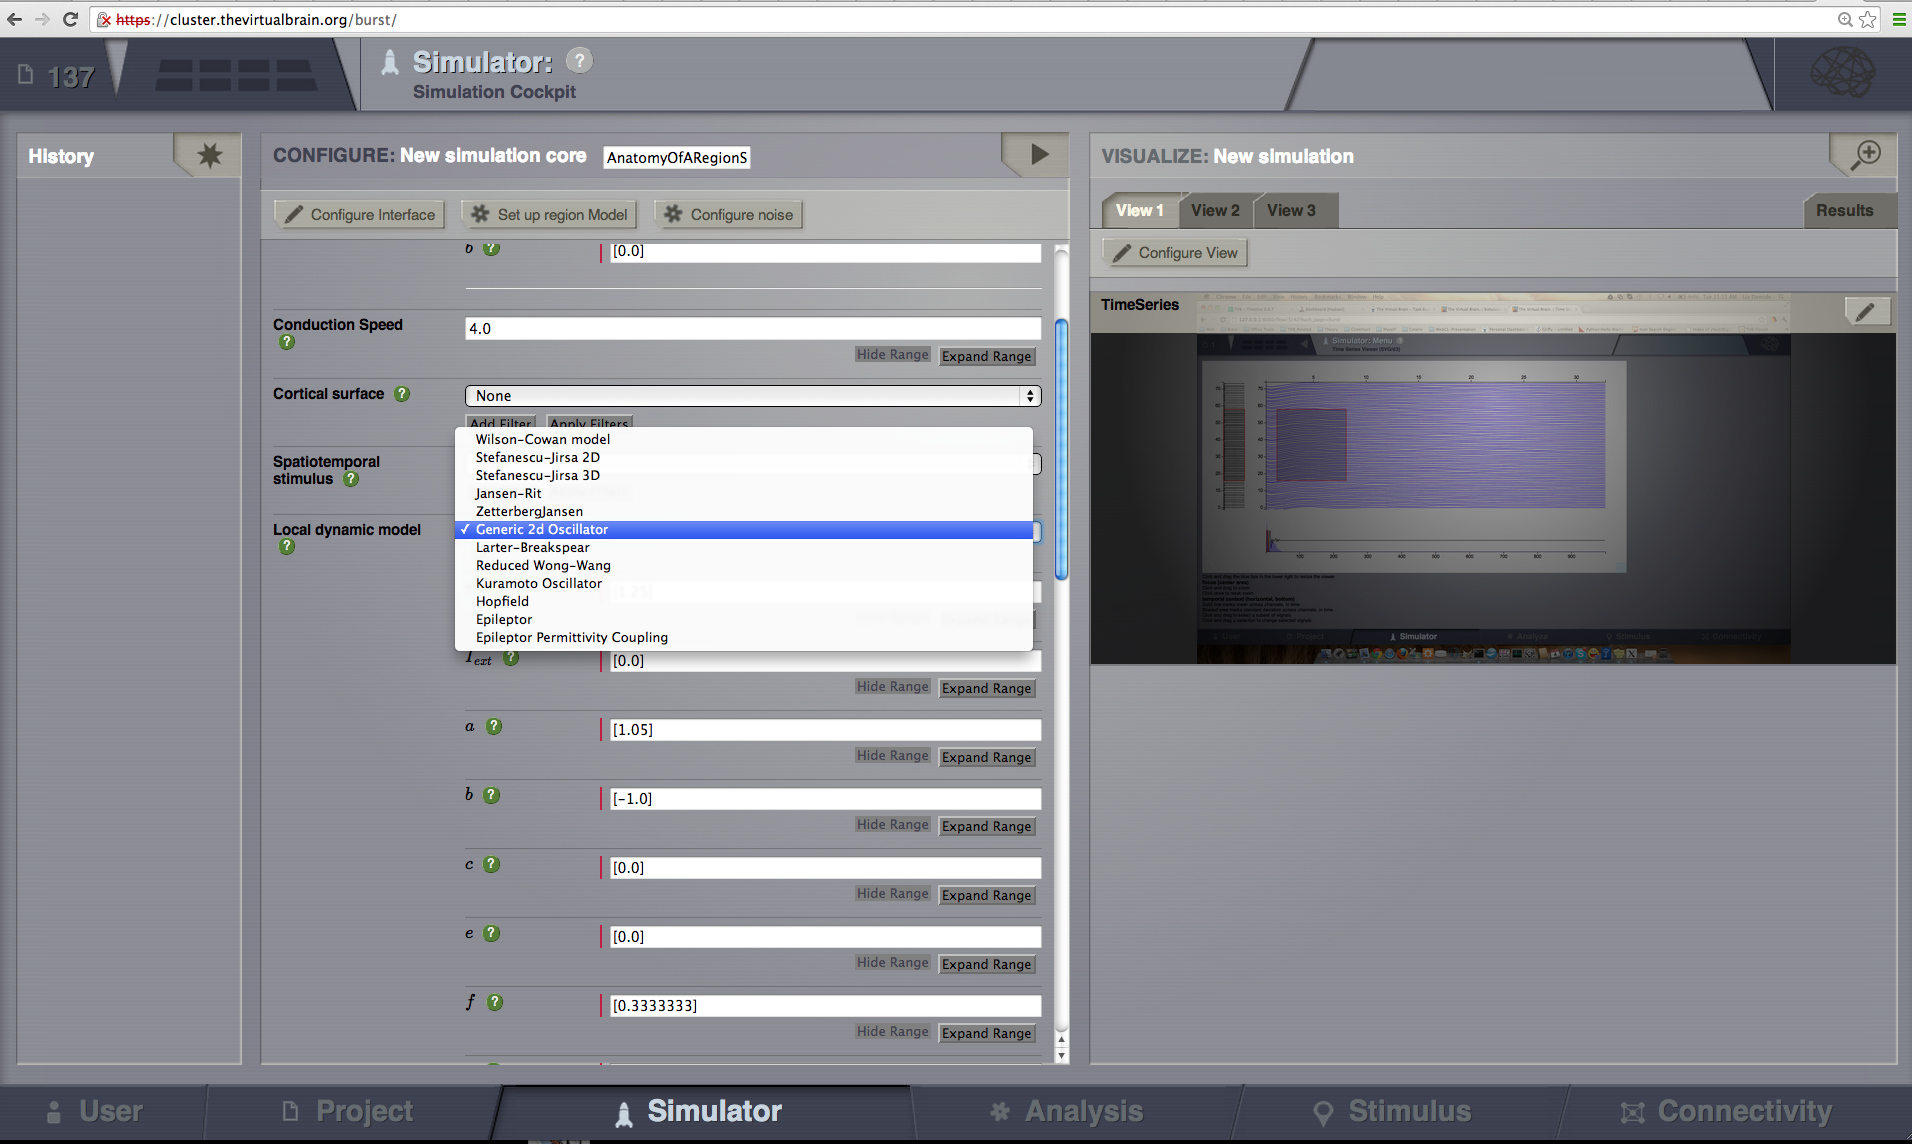
\includegraphics[width=\linewidth]{Handout_UI_BuildingYourOwnBrainNetworkModel_Model}%
  \caption{TVB Simulator page}%
  \label{fig:step_01}%
\end{figure}


\begin{margintable}
  \centering
  \fontfamily{ppl}\selectfont
  \begin{tabular}{ll}
    \toprule
    Model parameter & Value         \\
    \midrule
             $a$        &   1.05   \\
             $b$        &  -1.0    \\
             $c$        &   0      \\
             $d$        &   0.1    \\
             $e$        &   0      \\
             $f$        &   1/3    \\
             $g$        &   1      \\
             $I$        &   0      \\
             $\alpha$   &   1      \\
             $\beta$    &   0.2    \\
             $\gamma$   &  -1      \\
             $\tau$     &   1.25   \\
    \bottomrule
  \end{tabular}
  \caption{Generic 2d oscillator parameters}
  \label{tab:modeltab}
\end{margintable}



The important thing to know here is that TVB doesn't support interpolation of
the time-series it produces, which means that the period given to a monitor
must be an integral multiple of the time step size, \underline{dt}, selected for the integration scheme.
So, for our example the \underline{Monitor's} period is 1 ms. 
Although there are Monitors which apply a biophysical measurement process to
the simulated neural activity, such as EEG, MEG, etc, here we'll select only
one simple monitor just to show the idea. The \underline{Raw Monitor} takes no arguments
and simply returns all the simulated data. As a general rule this monitor
shouldn't be used for anything but very short simulations as the amount of
data returned can become prohibitively large.


\begin{simulation}
\begin{enumerate}[resume]
  \setcounter{enumi}{5}
 \item The last simulation configuration step is to provide the simulation length, that here we'll use the default value of 1000 ms.
 \item Before launching the simulation we can configure a set of visualizers and/or analyzers to have a glimpse of the results as soon as the simulation ends. It is possible to configure up to 12 different portlets. 
 \item And now we're ready to launch the simulation. 
\end{enumerate}
\end{simulation}


\subsection{Steps: Looking at the Results}\label{sec:steps}


The transient large amplitude oscillatory activity at the beginning of the
simulation is a result of the imperfectly set initial conditions -- they are
merely set by default to be random walks within the general range of state-
variable values expected from the model. As the current simulation is
configured with fixed point dynamics, if we were to set the initial conditions
exactly to the values corresponding to that fixed point there would be no such
initial transient (we will see how to achieve that later on).

\begin{formal}
\begin{enumerate}
\item Check the Fourier spectrum and select a linear scale on the Y axis. 
We see that the intrinsic frequency of the oscillations is set at about 11 Hz. 
\item Now let's have a look at a second simulation (\textit{AnatomyOfARegionSimulation\_b}) with the same parameters, except that the coupling strength has been increased by an order of magnitude (0.042). 
\end{enumerate}
\end{formal}

Looking at the time series, we can see that the system exhibits self-sustained
oscillations. A frequent question is at which value of coupling strength this
"bifurcation" occurs? Well, we can easily set up a parameter search by giving a
range of values to the coupling strength. TVB will launch a simulation for
every value. For the time being, parameter space explorations are restricted to
two dimensions.


\begin{simulation}
\begin{itemize}
 \item The example us set up in \textit{AnatomyOfARegionSimulation\_pse\_a}. One hundred and fifty (150) simulations of 2 seconds each were launched, each of them has the same underlying model, however two global parameters were explored: global coupling strength and conduction speed. These results are those shown in \citep{Ghosh_2008} and \citep{Knock_2009}. 
\end{itemize}
\end{simulation}


Let's see a few other parameters that could be adjusted. We mentioned before
that the big transient at the beginning is due to the initial conditions. To
overcome this issue we have a few alternatives. First, we could narrow the range of the state variables around the values of a fixed point. How do we know this value?

\begin{simulation}
\begin{enumerate}
\item  Clik on \underline{Set up region model}, you'll be redirected to a new working area.
\end{enumerate}
\end{simulation}


In this area there's a an interactive tool, which allows you to understand the
local dynamics by observing how the model parameters change the phase
plane. 


\begin{figure}[h]
  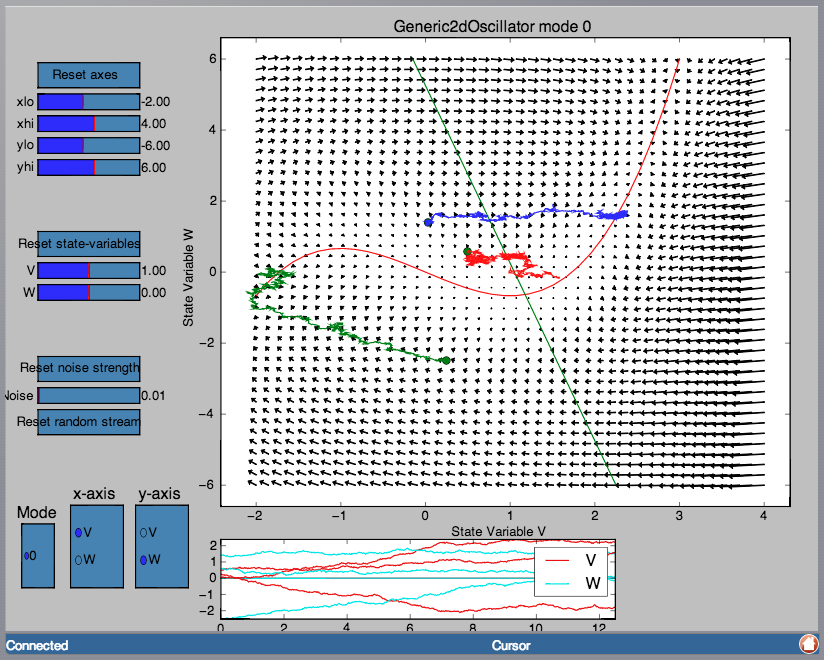
\includegraphics[width=\linewidth]{Handout_UI_BuildingYourOwnBrainNetworkModel_PPI}%
  \caption{Phase Plane Interactive}%
  \label{fig:ppi}%
\end{figure}

\begin{simulation}
\begin{enumerate}[resume]
  \setcounter{enumi}{1}
\item  Click on any point of the phase plane. A trajectory will be drawn.
We see that the fixed point is approx (V, W) = 1.5, -0.6
\end{enumerate}
\end{simulation}


However, there certainly is a more elegant way. 

\begin{simulation}
\begin{enumerate}[resume]
  \setcounter{enumi}{2}
\item Set your model with fixed point dynamics and a weak coupling strength.
\item Run a simulation for a few seconds.
\item TVB has a branching mechanism that allows you to use a previously run
simulation as the initial history for a new simulation. The only thing you
need to know is that the spatio-temporal structure of the network should
remain unchanged (eg, the number of nodes, speed, recorded state-variables,
integration time-step sizes and selected monitors should be the same.)
\end{enumerate}
\end{simulation}

\begin{simulation}
\begin{itemize}
 \item \textit{AnatomyOfARegionSimulation\_a\_branch1} is an example of this functionality, using the results from \textit{AnatomyOfARegionSimulation\_a} as initial conditions. Note that parameters should be modified before clicking on the branching icon.
\end{itemize}
\end{simulation}



As a last point, we will  show the basics of running a simulation driven by
noise (i.e., using a stochastic integration scheme). Here we'll also use a region
level simulation, but the considerations for surface simulations are the same.

In a stochastic (Noisy) integration scheme \underline{Noise} enters through the integration
scheme, here we'll define a simple constant level of noise that enters all
nodes and all state variables, however, the noise is configurable on a per
node and per state variable level, and as such the noise can be reconfigured
to, for example, only enter appropriate state variables of certain thalamic
nodes, thus emulating a very crude model of brain stem input to the brain. We
can choose between \underline{Additive} and \underline{Multiplicative Noise} functions when defining
the way noise enters our simulation. In the case of \underline{Multiplicative Noise} the
function depends on the state of the system. The \underline{Noise} functions are fed by a
random process generated by a pseudo-random number generator (PRNG). The random
processes used have Gaussian amplitude and can potentially be given a temporal
correlation (coloured noise). The random process is defined using two
parameters plus the seed of the PRNG. The two parameters are: \underline{D}, defining the
standard deviation of the noise amplitude; and \underline{$\tau$} which defines the
correlation time of the noise source, with $\tau = 0$ corresponding to white
noise and any value greater than zero producing coloured noise. The default
random seed is 42. Here, we'll specify a small amplitude white noise and pass
it into our stochastic integrator. As a general rule of thumb, the noise
amplitude, when being applied to all nodes and all state-variables, should be
much less than 1\% of the expected state-variable range if you don't want the
noise to dominate the intrinsic dynamics of the system.
If you are not sure about the level of Noise, using the Phase Plane
Interactive for plotting noisy trajectories is a good place to start.



(Screenshots of the PPI.)


\begin{simulation}
\begin{itemize}
 \item \textit{AnatomyOfARegionSimulation\_b\_branch1} and \textit{AnatomyOfARegionSimulation\_c} have the same parameters but the latter has an extra background noisy input. We can appreciate the differences in the \underline{Spectrogram of the Wavelet Transform}.
\end{itemize}
\end{simulation}


(Screenshots of wavelet spectrogram.)


\begin{simulation}
\begin{itemize}
 \item If you are already anxious and wondering about fMRI and some other biophysical output modalities in \textit{AnatomyOfARegionSimulation\_d} we've generated 8 minutes worth of data using a convolution based model of the BOLD signal. 
\end{itemize}
\end{simulation}


And that's it for this tutorial, while it's not a particularly scientifically
interesting simulation hopefully it gave you a sense of the anatomy of a
simulation within TVB and many of the configurable parameters and output
modalities.


\section{More Documentation}\label{sec:more-doc}
For more documentation on The Virtual Brain, please see the following articles \citep{Ghosh_2008}-Leon_2013, Spiegler_2013, Woodman_2014, Jirsa_2010b}


\section{Support}\label{sec:support}

The official TVB webiste is \url{www.thevirtualbrain.org}.  
All the documentation and tutorials are hosted on \url{the-virtual-brain.github.io}.
You'll find our public \smallcaps{git} repository at \url{https://github.com/the-virtual-brain}. 
For questions and bug reports we have a users group \url{https://groups.google.com/forum/#!forum/tvb-users}

\bibliography{tvb_references}
\bibliographystyle{plainnat}

\end{document}